% Options for packages loaded elsewhere
\PassOptionsToPackage{unicode}{hyperref}
\PassOptionsToPackage{hyphens}{url}
\documentclass[
  ignorenonframetext,
]{beamer}
\newif\ifbibliography
\usepackage{pgfpages}
\setbeamertemplate{caption}[numbered]
\setbeamertemplate{caption label separator}{: }
\setbeamercolor{caption name}{fg=normal text.fg}
\beamertemplatenavigationsymbolsempty
% remove section numbering
\setbeamertemplate{part page}{
  \centering
  \begin{beamercolorbox}[sep=16pt,center]{part title}
    \usebeamerfont{part title}\insertpart\par
  \end{beamercolorbox}
}
\setbeamertemplate{section page}{
  \centering
  \begin{beamercolorbox}[sep=12pt,center]{section title}
    \usebeamerfont{section title}\insertsection\par
  \end{beamercolorbox}
}
\setbeamertemplate{subsection page}{
  \centering
  \begin{beamercolorbox}[sep=8pt,center]{subsection title}
    \usebeamerfont{subsection title}\insertsubsection\par
  \end{beamercolorbox}
}
% Prevent slide breaks in the middle of a paragraph
\widowpenalties 1 10000
\raggedbottom
\AtBeginPart{
  \frame{\partpage}
}
\AtBeginSection{
  \ifbibliography
  \else
    \frame{\sectionpage}
  \fi
}
\AtBeginSubsection{
  \frame{\subsectionpage}
}
\usepackage{iftex}
\ifPDFTeX
  \usepackage[T1]{fontenc}
  \usepackage[utf8]{inputenc}
  \usepackage{textcomp} % provide euro and other symbols
\else % if luatex or xetex
  \usepackage{unicode-math} % this also loads fontspec
  \defaultfontfeatures{Scale=MatchLowercase}
  \defaultfontfeatures[\rmfamily]{Ligatures=TeX,Scale=1}
\fi
\usepackage{lmodern}
\ifPDFTeX\else
  % xetex/luatex font selection
\fi
% Use upquote if available, for straight quotes in verbatim environments
\IfFileExists{upquote.sty}{\usepackage{upquote}}{}
\IfFileExists{microtype.sty}{% use microtype if available
  \usepackage[]{microtype}
  \UseMicrotypeSet[protrusion]{basicmath} % disable protrusion for tt fonts
}{}
\makeatletter
\@ifundefined{KOMAClassName}{% if non-KOMA class
  \IfFileExists{parskip.sty}{%
    \usepackage{parskip}
  }{% else
    \setlength{\parindent}{0pt}
    \setlength{\parskip}{6pt plus 2pt minus 1pt}}
}{% if KOMA class
  \KOMAoptions{parskip=half}}
\makeatother
\usepackage{graphicx}
\makeatletter
\newsavebox\pandoc@box
\newcommand*\pandocbounded[1]{% scales image to fit in text height/width
  \sbox\pandoc@box{#1}%
  \Gscale@div\@tempa{\textheight}{\dimexpr\ht\pandoc@box+\dp\pandoc@box\relax}%
  \Gscale@div\@tempb{\linewidth}{\wd\pandoc@box}%
  \ifdim\@tempb\p@<\@tempa\p@\let\@tempa\@tempb\fi% select the smaller of both
  \ifdim\@tempa\p@<\p@\scalebox{\@tempa}{\usebox\pandoc@box}%
  \else\usebox{\pandoc@box}%
  \fi%
}
% Set default figure placement to htbp
\def\fps@figure{htbp}
\makeatother
\setlength{\emergencystretch}{3em} % prevent overfull lines
\providecommand{\tightlist}{%
  \setlength{\itemsep}{0pt}\setlength{\parskip}{0pt}}
\usepackage{bookmark}
\IfFileExists{xurl.sty}{\usepackage{xurl}}{} % add URL line breaks if available
\urlstyle{same}
\hypersetup{
  hidelinks,
  pdfcreator={LaTeX via pandoc}}

\author{\texorpdfstring{}{}}
\date{}

\begin{document}

\section{Categorical Semantics: DisCoCat and Compositional
Flow}\label{sec:categorical-semantics}

\begin{frame}{Two Traditions of Meaning: Formal and Distributional}
\protect\phantomsection\label{two-traditions-of-meaning-formal-and-distributional}
The study of linguistic meaning has long been divided between two
traditions with complementary strengths and weaknesses:

\begin{enumerate}
\item
  \textbf{Formal semantics}, following Montague
  {[}-@montague1973proper{]}, assigns meaning compositionally: the
  meaning of a complex expression is a function of the meanings of its
  parts and the way they are syntactically combined. This tradition
  excels at capturing logical structure (quantification, negation,
  modality) but struggles with lexical meaning---it typically treats
  content words as unanalyzed primitives.
\item
  \textbf{Distributional semantics} assigns meaning empirically: a
  word's meaning is characterized by its distribution across contexts,
  typically encoded as a vector in a high-dimensional space. The
  distributional hypothesis---``You shall know a word by the company it
  keeps'' {[}@firth1957papers{]}---traces to J.R. Firth's contextual
  theory of meaning and, independently, to Zellig Harris's
  {[}-@harris1954distributional{]} algebraic analysis of distributional
  structure, which demonstrated that linguistic elements occurring in
  similar environments share semantic properties. This tradition
  captures graded similarity and analogy but lacks compositional
  structure---the meaning of ``dog bites man'' and ``man bites dog'' may
  receive identical vector representations.
\end{enumerate}

The tension between these two traditions is one of the deepest in the
science of language. Turney and Pantel's {[}-@turney2010frequency{]}
comprehensive survey of vector space models showed that distributional
methods capture remarkably fine-grained semantic
distinctions---synonymy, antonymy, hypernymy, analogy---but only at the
word level. Baroni and Lenci {[}-@baroni2010distributional{]} developed
a tensor-based \emph{Distributional Memory} framework that partially
addresses compositionality by structuring co-occurrence data as a
three-way tensor over (word, relation, word) triples, but without a
principled type-logical backbone. Lenci {[}-@lenci2018distributional{]}
surveys the modern landscape and identifies the central open problem:
how to reconcile the \emph{algebraic compositionality} of formal
semantics with the \emph{empirical grounding} of distributional models.

The \textbf{DisCoCat} (Distributional Compositional Categorical)
framework {[}@coecke2010mathematical{]} resolves this tension by using
category theory to compose distributional meanings according to
syntactic structure---achieving, for the first time, a framework that is
simultaneously \emph{compositional} (from categorial grammar),
\emph{distributional} (from corpus-derived vector spaces), and
\emph{algebraically principled} (from monoidal category theory).
\end{frame}

\begin{frame}{From Static Embeddings to Contextual Representations: LLMs
as Distributional Models}
\protect\phantomsection\label{from-static-embeddings-to-contextual-representations-llms-as-distributional-models}
The distributional programme has undergone a dramatic computational
intensification in the era of large language models (LLMs). The
trajectory from classical co-occurrence matrices through static word
embeddings to contextual transformers can be understood as a progressive
\emph{enrichment} of the distributional hypothesis itself:

\begin{enumerate}
\item
  \textbf{Static embeddings}: Mikolov et al.'s
  {[}-@mikolov2013efficient{]} Word2Vec (skip-gram and CBOW
  architectures) demonstrated that prediction-based training on local
  context windows produces word vectors exhibiting striking algebraic
  regularity---the famous ``king \(-\) man \(+\) woman \(\approx\)
  queen'' analogy. Pennington et al.'s {[}-@pennington2014glove{]} GloVe
  incorporated global co-occurrence statistics via log-bilinear
  regression, yielding vectors whose inner products approximate
  pointwise mutual information. Both models instantiate the
  distributional hypothesis in its classical Firthian form: meaning is
  determined by context of use, encoded as geometric position in a
  learned vector space.
\item
  \textbf{Contextual embeddings}: BERT {[}@devlin2019bert{]} and GPT
  {[}@radford2018improving{]} move beyond static type-level
  representations to \emph{token-level} contextualized embeddings, where
  the same word receives different vectors in different contexts. In the
  terms of the formal/distributional dichotomy, this is a critical
  advance: contextualized embeddings partially capture
  \emph{compositional} structure by conditioning word representations on
  their full sentential environment, resolving polysemy and
  constructional effects that static embeddings conflate.
\item
  \textbf{Transformer architecture}: The transformer
  {[}@vaswani2017attention{]} implements distributional composition
  through multi-head self-attention, where each attention head computes
  a weighted combination of input token representations. The attention
  weights \(\alpha_{ij} = \text{softmax}(Q_i K_j^T / \sqrt{d_k})\) are
  analogous to the enriched hom-values of
  \autoref{sec:enriched-categories}: they encode the \emph{degree of
  contextual relevance} between tokens \(i\) and \(j\) in a given
  representational subspace---a graded, learned distributional relation.
\end{enumerate}

The connection to our categorical framework is direct: \textbf{DisCoCat
is the algebraic formalization of what LLMs do empirically.} Where a
transformer computes sentence representations by attending to
syntactically and semantically relevant tokens through learned weight
matrices, DisCoCat composes word vectors through type-logical
derivations in a compact closed category. The functor
\(F: \mathbf{Preg} \to \mathbf{FVect}\) that defines DisCoCat is, in
this light, the \emph{principled version} of the composition that
attention mechanisms learn from data. This perspective is confirmed by
Gavranović's {[}-@gavranovic2024thesis{]} categorical deep learning
programme, which shows that attention heads can be understood as
parameterized optics---categorical constructions that compose
functorially, just as DisCoCat derivations do.

For case theory specifically, the transformer analogy is illuminating:
each attention head in a transformer can be understood as learning a
particular \emph{relational role}---attending to subjects, objects,
modifiers, or other grammatical functions. This is precisely the role
that case marking plays in natural language: structuring
who-does-what-to-whom. The case-typed noun spaces of our enriched
DisCoCat model
(\(N_{\text{NOM}}, N_{\text{ACC}}, N_{\text{DAT}}, \ldots\)) correspond
to the role-specific representational subspaces that different attention
heads learn to inhabit.
\end{frame}

\begin{frame}{The DisCoCat Compositional Framework}
\protect\phantomsection\label{the-discocat-compositional-framework}
\begin{block}{The Key Insight: Shared Compact Closed Structure}
\protect\phantomsection\label{the-key-insight-shared-compact-closed-structure}
DisCoCat's central observation is that pregroup grammars and vector
spaces share a common abstract structure: both are \textbf{compact
closed categories}. This means there exists a \emph{meaning functor}:

\[F: \mathbf{Preg} \to \mathbf{FVect} \] \{\#eq:eq-4-1\}

from the pregroup grammar category (where objects are types and
morphisms are grammatical reductions) to the category of
finite-dimensional vector spaces (where objects are vector spaces and
morphisms are linear maps).

Under this functor:

\begin{itemize}
\tightlist
\item
  Noun types \(n\) map to a vector space \(N\) (the noun space)
\item
  Sentence types \(s\) map to a vector space \(S\) (the sentence space)
\item
  A transitive verb of type \(n^r \cdot s \cdot n^l\) maps to a tensor
  in \(N \otimes S \otimes N\)
\item
  Pregroup contractions (cups/caps) map to the standard inner product
  and its dual
\end{itemize}
\end{block}

\begin{block}{Computing Compositional Sentence Meaning}
\protect\phantomsection\label{computing-compositional-sentence-meaning}
The compositional meaning of a sentence is computed by tensoring the
word meanings and then contracting the result along the indices
determined by the syntactic derivation. For ``Alice chases Bob'':

\[\overrightarrow{\text{Alice chases Bob}} = (\overrightarrow{\text{Alice}} \otimes \overleftrightarrow{\text{chases}} \otimes \overrightarrow{\text{Bob}}) \circ (\varepsilon_N \otimes 1_S \otimes \varepsilon_N) \]
\{\#eq:eq-4-2\}

where \(\varepsilon_N: N \otimes N \to \mathbb{R}\) is the compact
closure map (inner product). This computation has a direct diagrammatic
representation as a string diagram---the same Joyal--Street
{[}@joyalstreet1991geometry{]} formalism that governs the syntax.
\end{block}

\begin{block}{Empirical Validation and Disambiguation}
\protect\phantomsection\label{empirical-validation-and-disambiguation}
Grefenstette and Sadrzadeh {[}-@grefenstette2015concrete{]} demonstrated
that DisCoCat models can outperform purely distributional baselines on
disambiguation and sentence similarity tasks. The key advantage is that
compositional structure resolves ambiguities that bag-of-words models
cannot: ``dog bites man'' and ``man bites dog'' receive different
sentence vectors because the syntactic structure assigns different roles
to the nouns.

\textbf{Attention as Cup contraction.} The claim that DisCoCat provides
the ``algebraic formalization'' of transformer-based LLMs can be made
precise. In a transformer's self-attention mechanism, the query--key
inner product \(\text{softmax}(QK^\top / \sqrt{d})V\) selects which word
vectors interact---effectively implementing a \emph{soft} version of the
Cup contraction. The pregroup Cup \(\varepsilon: n^r \otimes n \to I\)
contracts two noun wires into a scalar; the attention inner product
\(q_i \cdot k_j\) contracts two contextualized vectors into an attention
weight, which then mixes the value vectors. The difference is that the
DisCoCat Cup is \emph{binary} (either the types match or they don't)
while the attention Cup is \emph{graded} (producing a real-valued
weight). This is precisely the \([0,1]\)-enrichment of
\autoref{sec:enriched-categories} applied to the type-reduction level:
each attention head learns an enriched Cup that contracts types with
learned confidence weights rather than categorical yes/no type-matching.
Multi-head attention then corresponds to the tensor product of \(h\)
independent enriched contraction maps, each attending to a different
substring of the relational structure---analogous to how DisCoCat
composes multiple Cup contractions for multi-argument verbs.

\begin{figure}
\centering
\pandocbounded{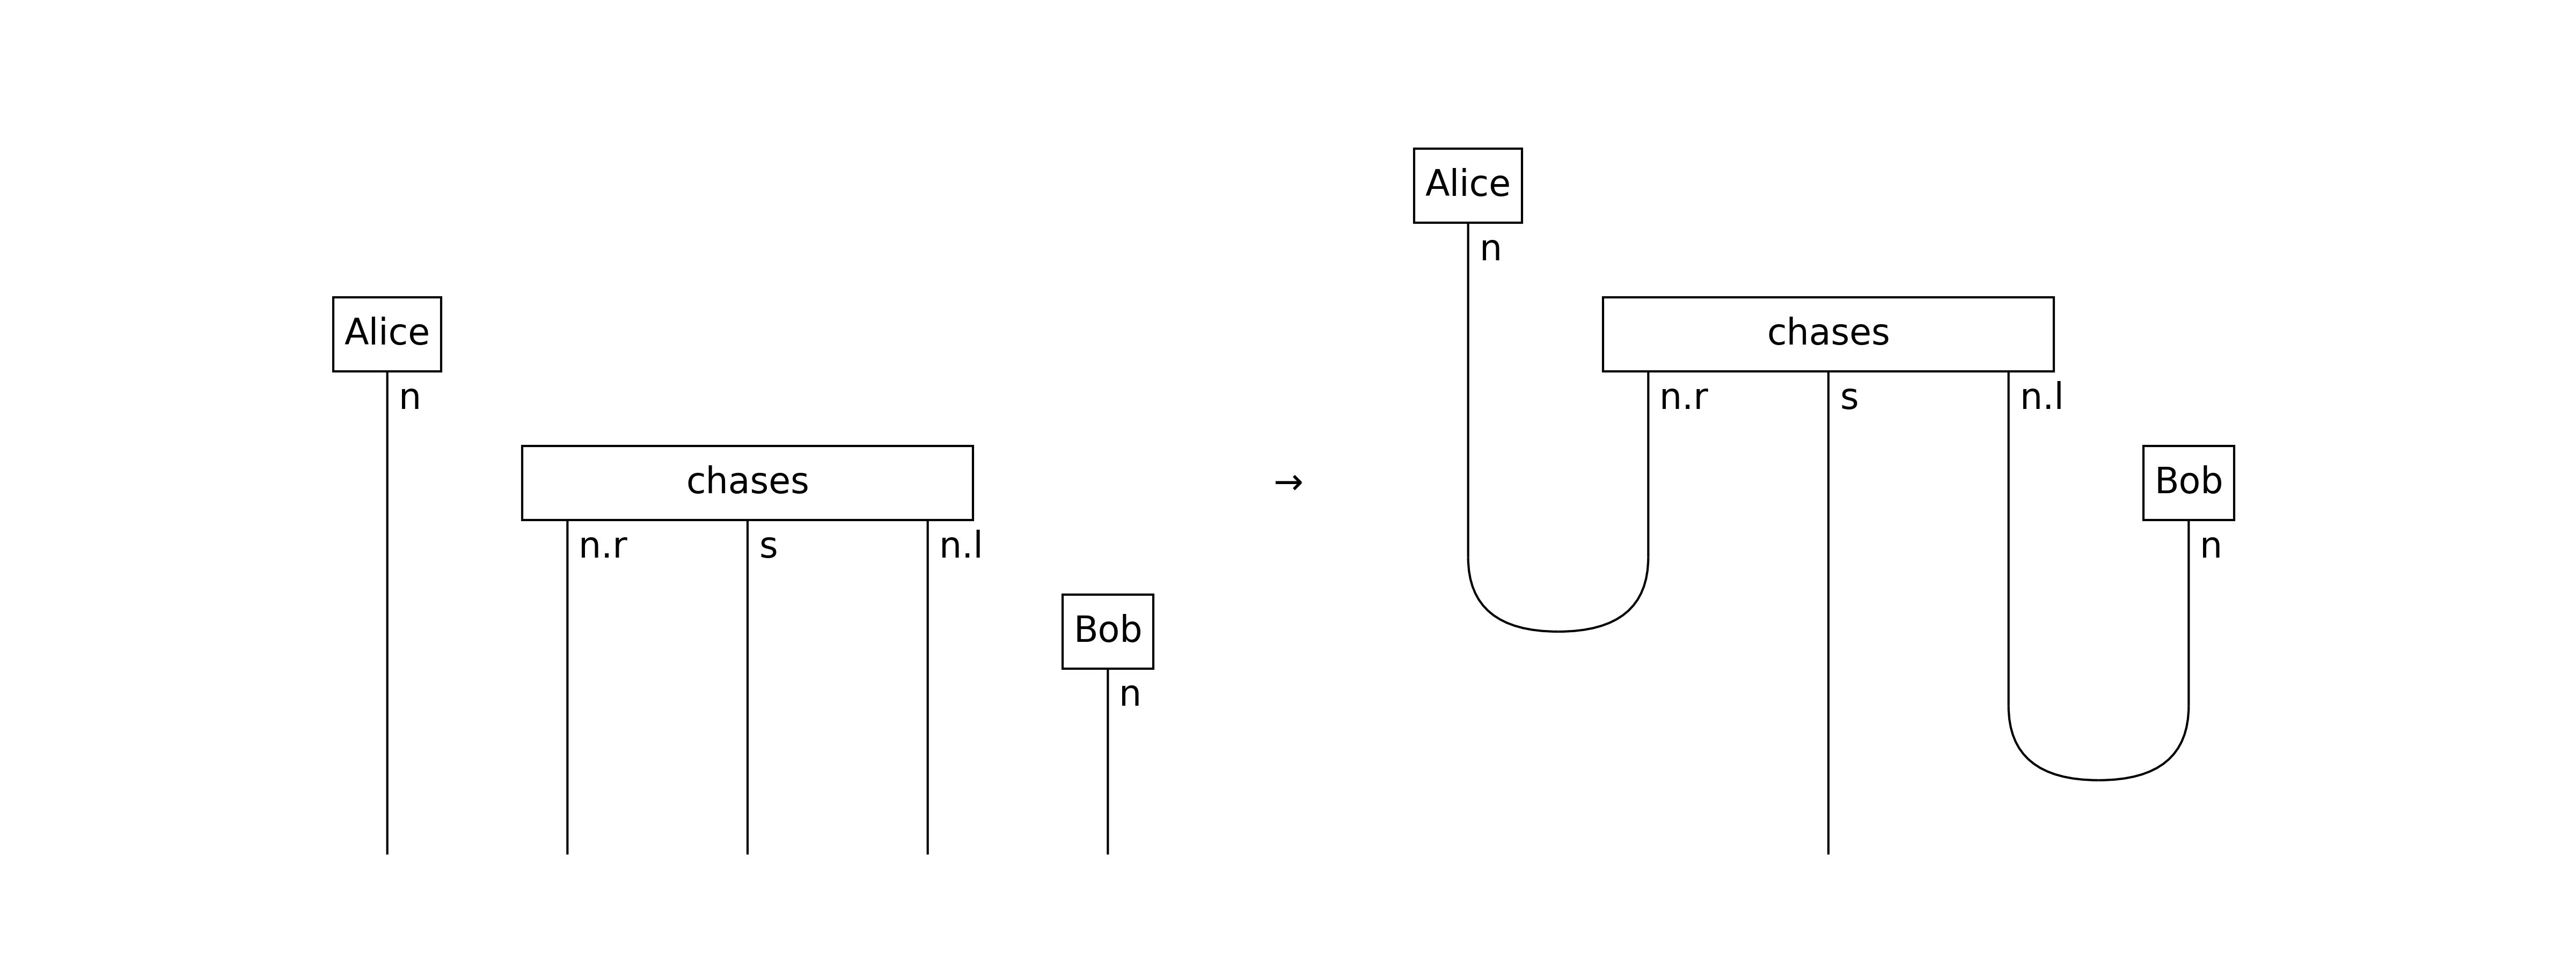
\includegraphics[keepaspectratio,alt={The compositional semantics of ``Alice chases Bob'' under the DisCoCat meaning functor F: \textbackslash mathbf\{Preg\} \textbackslash to \textbackslash mathbf\{FVect\}. The syntactic diagram (left of the functor) assigns pregroup types---n for nouns, n\^{}r \textbackslash otimes s \textbackslash otimes n\^{}l for the transitive verb---while F maps these to vector spaces: n \textbackslash mapsto N (noun space), s \textbackslash mapsto S (sentence space), and the verb's type to a tensor \textbackslash overleftrightarrow\{\textbackslash text\{chases\}\} \textbackslash in N \textbackslash otimes S \textbackslash otimes N. The Cup contractions become inner products \textbackslash varepsilon\_N: N \textbackslash otimes N \textbackslash to \textbackslash mathbb\{R\}, computing the sentence vector \textbackslash overrightarrow\{\textbackslash text\{Alice chases Bob\}\} \textbackslash in S by contracting the word tensors along syntactically determined indices.}]{../figures/discopy_composition.png}}
\caption{The compositional semantics of ``Alice chases Bob'' under the
DisCoCat meaning functor \(F: \mathbf{Preg} \to \mathbf{FVect}\). The
syntactic diagram (left of the functor) assigns pregroup types---\(n\)
for nouns, \(n^r \otimes s \otimes n^l\) for the transitive verb---while
\(F\) maps these to vector spaces: \(n \mapsto N\) (noun space),
\(s \mapsto S\) (sentence space), and the verb's type to a tensor
\(\overleftrightarrow{\text{chases}} \in N \otimes S \otimes N\). The
Cup contractions become inner products
\(\varepsilon_N: N \otimes N \to \mathbb{R}\), computing the sentence
vector \(\overrightarrow{\text{Alice chases Bob}} \in S\) by contracting
the word tensors along syntactically determined
indices.}\label{fig:discopy-discocat}
\end{figure}
\end{block}
\end{frame}

\begin{frame}{Case Enrichment in the DisCoCat Framework}
\protect\phantomsection\label{case-enrichment-in-the-discocat-framework}
The present contribution lies in showing how case marking enriches the
DisCoCat framework with explicit role structure. In a case-marked
DisCoCat model:

\begin{enumerate}
\item
  \textbf{Typed noun spaces}: Instead of a single noun space \(N\), we
  define case-specific spaces
  \(N_{\text{NOM}}, N_{\text{ACC}}, N_{\text{DAT}}, \ldots\) Morphisms
  between these spaces encode case-changing operations (passivization,
  dative shift, etc.).
\item
  \textbf{Case-constrained composition}: The meaning functor \(F\) maps
  case-typed pregroup derivations to tensor contractions that respect
  case constraints. A verb seeking a nominative subject and accusative
  object contracts only with vectors from the appropriate spaces.
\item
  \textbf{Alignment as Natural Transformation}: Cross-linguistic
  alignment differences correspond to different meaning functors.
  However, we go further by modeling case alignment as \textbf{natural
  transformations} between functors. An accusative-language
  transformation \(\eta_{\text{acc}}: \mathcal{I} \to F_{\text{acc}}\)
  identifies S and A arguments; an ergative transformation
  \(\eta_{\text{erg}}\) identifies S and P. This categorification allows
  us to model ``grammar'' as the requirement that these transformations
  commute with the DisCoCirc entity wires, ensuring role persistence
  across sentences.
\end{enumerate}

\begin{figure}
\centering
\pandocbounded{\includegraphics[keepaspectratio,alt={A 20-word DisCoPy pregroup grammar. This diagrammatic transparency exemplifies Shimojima's {[}-@shimojima1996reasoning{]} free-ride inference: by inspecting the diagram, one can immediately see that passivization preserves the verb's inherent argument structure while rearranging the surface realization---a fact that requires multiple inference steps to establish in a linear notation. Three dense noun phrases (with 4, 4, and 8 chained adjective modifiers respectively) reduce into the ditransitive verb's type n\^{}r \textbackslash otimes s \textbackslash otimes n\^{}l \textbackslash otimes n\^{}l via 4 Cup contractions, mapping 20 lexical items into the unified sentence type s. The resulting complexity score ({[}@eq:eq-4-4{]} in ) substantially exceeds that of simple transitive sentences, confirming the monotonic relationship between argument structure and derivational depth.}]{output/figures/discopy_ditransitive.png}}
\caption{A 20-word DisCoPy pregroup grammar. This diagrammatic
transparency exemplifies Shimojima's {[}-@shimojima1996reasoning{]}
free-ride inference: by inspecting the diagram, one can immediately see
that passivization preserves the verb's inherent argument structure
while rearranging the surface realization---a fact that requires
multiple inference steps to establish in a linear notation. Three dense
noun phrases (with 4, 4, and 8 chained adjective modifiers respectively)
reduce into the ditransitive verb's type
\(n^r \otimes s \otimes n^l \otimes n^l\) via 4 Cup contractions,
mapping 20 lexical items into the unified sentence type \(s\). The
resulting complexity score ({[}@eq:eq-4-4{]} in
\autoref{sec:compact-closure-discourse}) substantially exceeds that of
simple transitive sentences, confirming the monotonic relationship
between argument structure and derivational
depth.}\label{fig:discopy-ditransitive}
\end{figure}

The following sections extend this model to discourse and quantum
computation.
\end{frame}

\end{document}
